%!TEX root = ../thesis.tex

\chapter{Background}\label{chapter:background}

This chapter introduces the background knowledge that necessary to understand the project and why it has been developed.
It first establishes the concept of Internet of Things, which is at the base of this thesis, afterwards, it describes the problem statement and gives an overview on the background work and state of the art present at the moment of writing.

% A deeper understanding of the related work can be found in chapter Related Work.

\section{Internet of Things}

The \textit{Internet of Things}, abbreviated with \textit{IoT}, has a longer history than many people know.

% Slide 9 corso internet of things helsinki 

% https://www.thoughtco.com/bar-codes-history-1991329
One of the first technologies that can be associated to IoT is the ``\textit{Universal Product Code}'', or \textit{UPC}.
% todo cambiare / modificare 
This was issued to inventors Joseph Woodland and Bernard Silver on October 7, 1952, and can be described as a ``bull's eye'' symbol, made up of a series of concentric circles \cite{upc_patent}. 

\begin{figure}
	\centering
	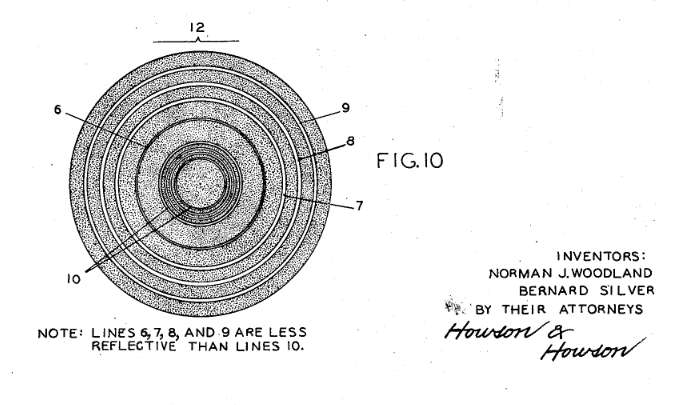
\includegraphics[width=\textwidth-3cm]{resources/img/upc_1}
	\caption{}
\end{figure}

Due to the large size of equipment and the scarse reliability, it has not been immediately introduced to the public.

The barcode was first used commercially in 1966, however, it was soon realized that there would have to be some sort of industry standard set.

The first appearance of the Universal Product Code (UPC) that is known to the public and has become widespread, is the one developed in 1971 by George Laurer at IBM.
\cite{upc_ibm}.

% TODO cambiare
Adoption relied on emergence of laser optics, developed around the same time, as these offered compact reading technology

Although, printers used to generate barcodes were vulnerable to smudge è design coped with errors as ink bleeding would result in taller bars.
Offered the first way to track products and	address them!

% TODO IMPORTANTE

Visto che le stampanti hanno cominciato ad essere vendute in larga scala e le stampe dunque costavano poco, l'adozione dell'UPC è stata addottata su larga scala.
GUARDARE SLIDE ECONOMIA DELL'INNOVAZIONE

% Slide 10 corso internet of things helsinki 

% 		Universal Product Code (UPC)
% 		• Developed in 1971 by George Laurer at IBM
% 		• Still in widespread use
% 		• Adoption relied on emergence of laser optics,
% 		developed around the same time, as these
% 		offered compact reading technology
% 		• Printers used to generate barcodes were
% 		vulnerable to smudge è design coped with errors as ink bleeding would result in taller
% 		bars
% 		• Offered the first way to track products and
% 		address them!


% https://www.engineersrule.com/how-a-coke-machine-and-the-industrial-internet-of-things-can-give-birth-to-a-planetary-computer/
% https://www.ibm.com/blogs/industries/little-known-story-first-iot-device/
% https://www.cs.cmu.edu/~coke/history_long.txt
It may come as a surprise, but connecting everyday objects has started in 1980 - mid 90s.
One of the most famous and most quoted as the is the first IoT device, is the Carnegie Mellon University (CMU) coke machine at the Computer Science Department.

This used sensors to detect whether shelves have bottles.
Simple algorithms used to track status of coke bottles (warm, cold, empty).
Allow remote access to check status of machine.
Communication took place through Arpanet at CMU as the system predated the Internet.

%		Slide 11

%	https://www.smithsonianmag.com/innovation/kevin-ashton-describes-the-internet-of-things-180953749/
%	http://www.itrco.jp/libraries/RFIDjournal-That%20Internet%20of%20Things%20Thing.pdf
%	https://www.rfidjournal.com/that-internet-of-things-thing
The term ``\textit{Internet of Things}'' which is now know all around the globe, has been attributed to \textit{Kevin Ashton}, who used it in a presentation at \textit{Protector \& Gamble} in 1999 \cite{iot_definition} to describe the network connecting objects in the physical world to the Internet.

IOT TRENDS AND FORECASTS

% https://www.fintechnews.org/top-emerging-iot-trends-business-should-look-for-in-2021/
% https://www.forbes.com/sites/danielnewman/2020/11/25/5-iot-trends-to-watch-in-2021/
% https://www.siemens-advanta.com/blog/what-are-expected-iot-trends-2021

Another important definition of IoT is IIoT, which stands for Industri 4.0 IoT.

\section{Air quality}

% Describe the problem with air quality, link some papers that show that it has been getting worse in the last decades
% Show that there are standards to measure air quality		
% Say something about air quality in the covid era (covid has helped people re-evaluate the use of bikes and other publicly-shared methods of transportation)
% Stopping, although painful for the society (physically and economically) has helped demonstrating that there is still hope to get a clean environment in which to live

% TODO mantenere le sezioni succesive in questo capitolo o spostare nel successivo?

The solution this thesis focuses on is MegaSense

\section{Solutions to detect air pollution}

% Describe these solutions, history, pricing (from the ones that cost a lot and are very reliable to the ones that are cheap and less reliable; a high amount of cheap devices can perform almost as good as a high end device)
% Describe some solutions that have been previously proposed by other researchears and universities

ArduECO

\begin{figure}
	\centering
	\includegraphics[width=\textwidth]{resources/img/ardueco_circuit}
	\caption{}
\end{figure}

\begin{figure}
	\centering
	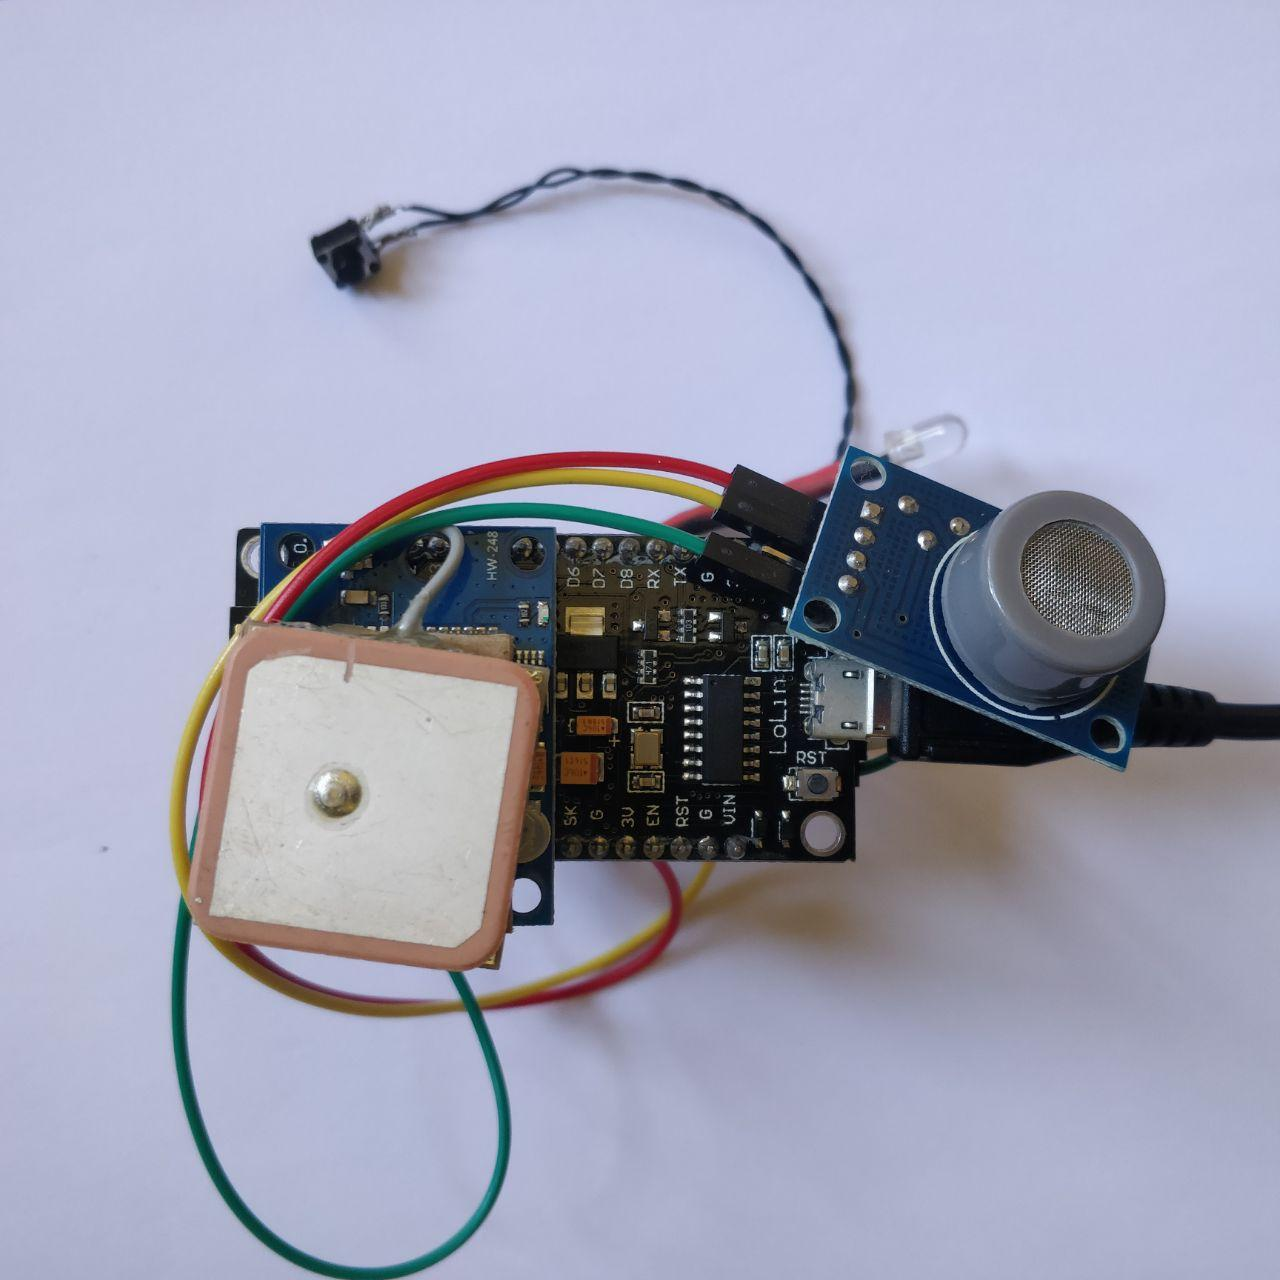
\includegraphics[width=.5\textwidth]{resources/img/ardueco_picture}
	\caption{}
\end{figure}

\section{\megasense}\label{sec:megasense}

% Describe the megasense project, put pictures and explain how it has been developed until now

https://www.megasense.org/

Describe the consortium

HOPE and Megasense

The calibration of the megasense device is made via